% mainfile: ../../../../master.tex
\subsection{Macromolecular composition of cells with R}
% The part of the label after the colon must match the file name. Otherwise,
% conditional compilation based on task labels does NOT work.
\label{task:20180303_cj0}
\tags{dna,rna,r}
\authors{cj}
%\files{}
%\persons{}

Because I had surprising results regarding my yields of DNA and RNA, I decide to learn a little bit more about the proportions of macromolecules in cells and to try to represent it with diagrams.


\citet{finkel2016phylogenetic}

After reading a \href{http://book.bionumbers.org/what-is-the-macromolecular-composition-of-the-cell/}{webpage} related to the article by \citet{milo2009bionumbers}, 

\begin{lstlisting}[language=r, caption=Waffle plots to represent the macromolecular composition of different type of cell, label=lst:20180303_rscript_waffle_plots]

img.path = "/Users/Clara/Projects/diary/graphics/plots/"
today <- "20180303"
# http://book.bionumbers.org/what-is-the-macromolecular-composition-of-the-cell/
ecoli <- c(
	`protein`=55,
	`other`=22,
	`RNA`=20,
	`DNA`=3
	
	# `lipid`=9,
	# `lipopolysaccharide`=3,
	# `peptidoglycan`=3,
	# `glycogen`=3,
	# `metabolites`=3,
	# `inorganic ions`=1
	)

purple.palette <- c("#cba7bc",
"#8a99d8",
"#d68dc0",
"#a7a6c8")

pdf(file = paste(img.path, today, "_waffle_ecoli.pdf", sep="", collapse=NULL), width=4, height=4)
waffle(ecoli, 
	title = "Echerichia coli", 
	colors=purple.palette)
dev.off()

# Phylogenetic Diversity in the Macromolecular Composition of Microalgae
cyanobacteria <- c(
	`protein`=43,
	`other`= 47,
	`RNA`=9,
	`DNA`=1
	#`lipid`=12,
	#`carbohydrates`=22,
	#`ash`=8,
	#`chlorophyll a`=1,
	#`other`=4
	)

cyano.palette <- c("#76a9d6",
"#58cbc0",
"#92b7bb",
"#4abdd8")

pdf(file = paste(img.path, today, "_waffle_cyano.pdf", sep="",  collapse=NULL), width=4, height=4)
waffle(cyanobacteria, 
	title = "Cyanobacteria", 
	colors=cyano.palette)
dev.off()

chlorophyta <- c(
	`protein`=33,
	`other`= 61,
	`RNA`=5,
	`DNA`=1
	)

chloro.palette <- c("#5dc5cd",
"#a7bf76",
"#9ebba8",
"#74c39e")

pdf(file = paste(img.path, today, "_waffle_chlorophyte.pdf", sep="", collapse=NULL), width=4, height=4)
waffle(chlorophyta, 
	title = "Chlorophyta", 
	colors=chloro.palette)
dev.off()

\end{lstlisting}

The script in listing \ref{lst:20180303_rscript_waffle_plots} generate waffle plots that are shown in figure \ref{fig:20180303_waffle_plots}.

\begin{figure}[H] % position of the figure 
    \centering
    \caption{Representation of the taxonomic differences of the median macromolecular composition as percent dry weight under nutrient-sufficient exponential growth conditions.}
    \label{fig:20180303_waffle_plots}
    \begin{subfigure}[b]{0.3\textwidth}
        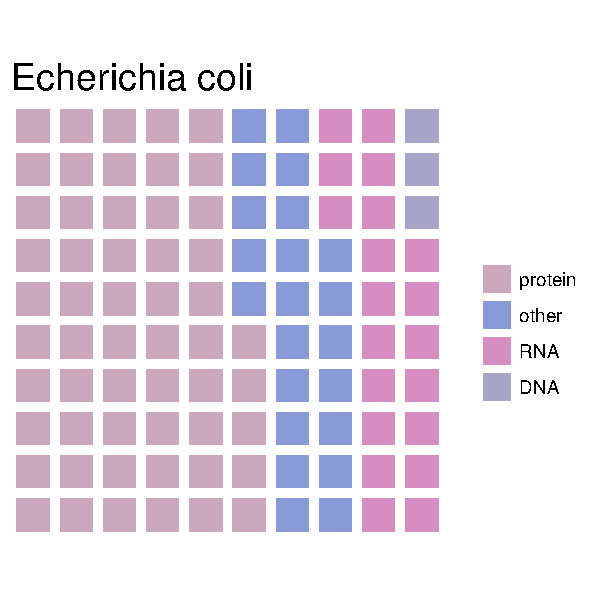
\includegraphics[width=\textwidth]{graphics/plots/20180303_waffle_ecoli.pdf}
        \caption{Bacteria (\textit{Echerichia coli})}
        \label{sfig:slabel1}
    \end{subfigure}
    ~ 
    \begin{subfigure}[b]{0.3\textwidth}
        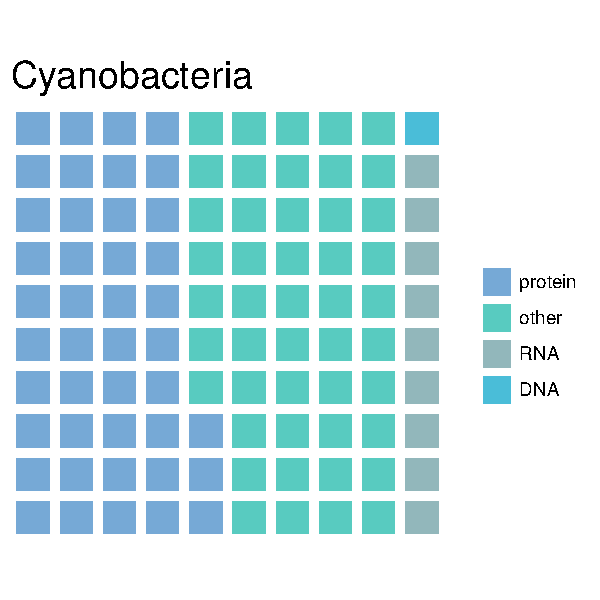
\includegraphics[width=\textwidth]{graphics/plots/20180303_waffle_cyano.pdf}
        \caption{Bacteria (cyanobacteria)}
        \label{sfig:slabel2}
    \end{subfigure}
    ~
    \begin{subfigure}[b]{0.3\textwidth}
        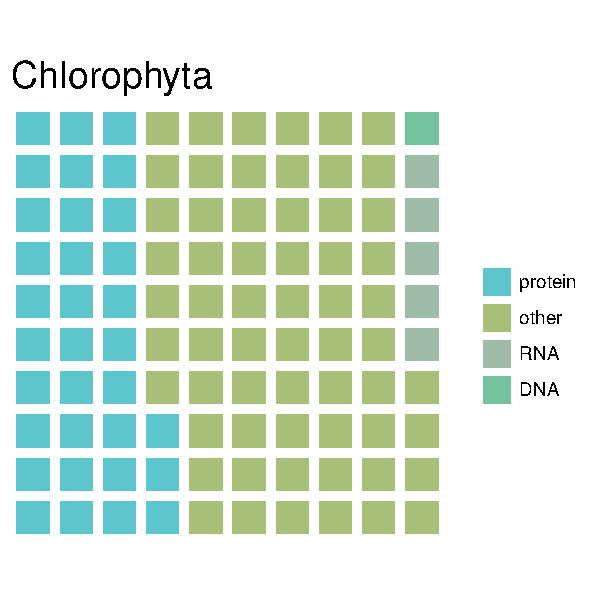
\includegraphics[width=\textwidth]{graphics/plots/20180303_waffle_chlorophyte.pdf}
        \caption{Eukaryote (\textit{Chlorophyta sp.})}
        \label{sfig:slabel2}
    \end{subfigure}
\end{figure}

